% !TEX root = sum1.tex
\section{Problem Description}

\subsection{Basic Concept}

At first, we will introduce some preliminary knowledge about our problem as follows.

We consider a set of groups to be assigned to a set of seats $S$. For the purpose of illustration, we consider the layout of $S$ as a rectangle formed by $m$ rows and $n$ columns. But our model and formulation allow for a more general layout of the seats. 

The customers from the same group can sit together while different groups should sit with the social distancing. Considering the actual situation, the social distancing is one seat in our paper and different rows have no effect each other, i.e., a person from one group can sit directly behind a person from another group.

For dealing with the social distancing together, we add one to the original size of each group as the new size of the group and one dummy seat to each row. Then the seat assignment for one row can be illustrated as below. 

\begin{figure}[ht]
    \centering
    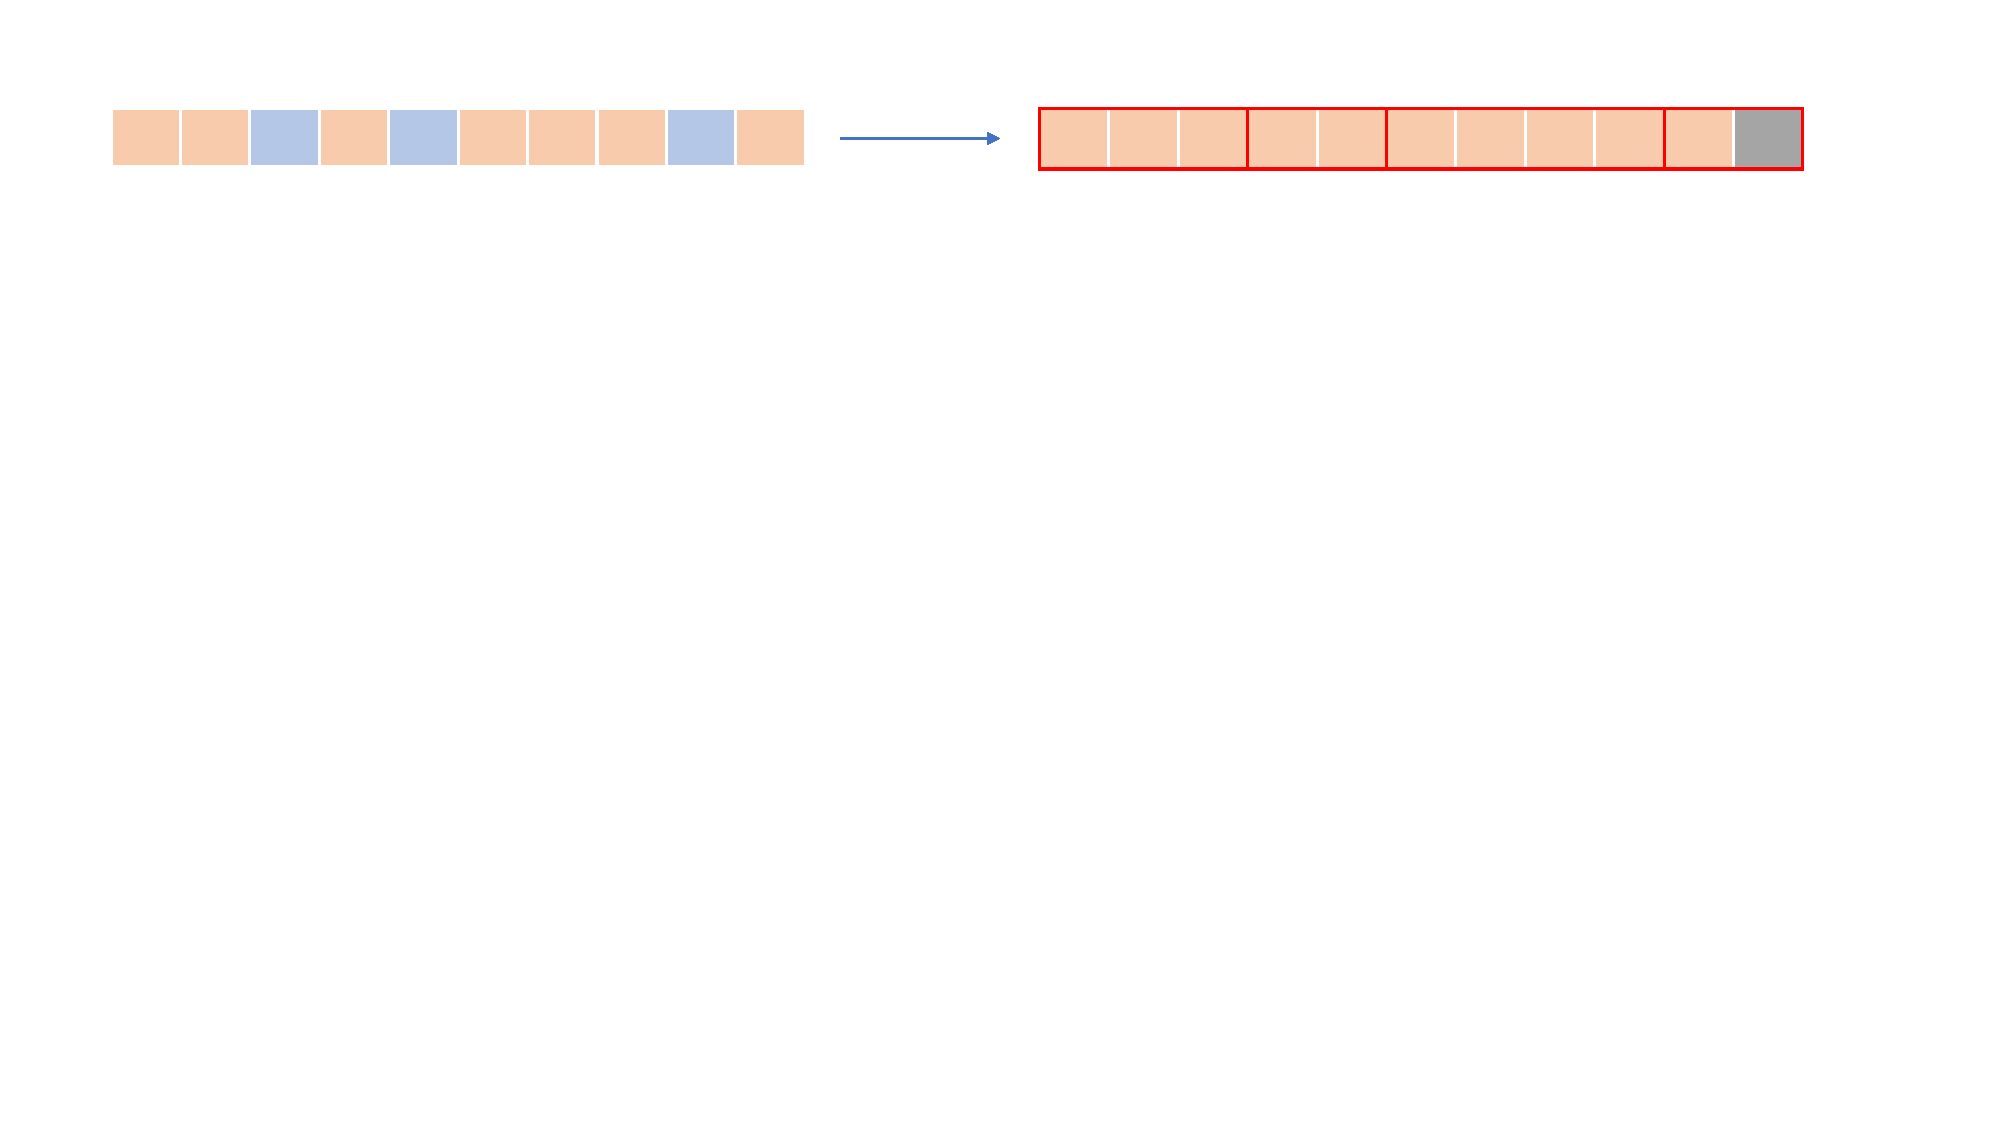
\includegraphics[width = 0.8\textwidth]{./Figures/dummy_seat.pdf}
    \caption{Problem Conversion}
\end{figure}

On the left side, the blue squares stand for the empty seats as the social distancing. The orange squares represent the seats sat by the groups. 
On the right side, one dummy seat is added at the end of the row. The orange squares surrounded by the red line are the seats taken by groups.

In this way, the social distancing will be integrated by solving this new seat assignment problem.

% The number of all seats in each row is called the length of the row.

\subsection{Deterministic Model}

We are given a demand, for example, $(d_1, d_2, d_3, d_4, d_5, d_6) = (3,5,7,0,10,6)$, where $d_i$ indicates the number of group containing $i$ people. Suppose each group has to leave a seat to maintain social distancing with the adjacent groups. Regard the groups as items in the CSP, and rows as stocks to be cut.

Suppose that the number of rows is fixed, we hope to accommodate as many as people possible.

And the IP formulation can be shown as below:

\begin{equation}\label{deter_upper}
    \begin{aligned}
      \max \quad & \sum_{j =1}^{N} \sum_{i = 1}^{m} (s_i -1) x_{ij} \\
      \text {s.t.} \quad & \sum_{i = 1}^{m} s_i x_{ij} \leq L_{j}, j=1,\ldots,N \\
      & \sum_{j =1}^{N} x_{ij} \leq d_{i}^{u}, i=1,\ldots,m \\
      & x_{ij} \geq 0, i=1,\ldots,m, j=1,\ldots,N.
    \end{aligned}
\end{equation}

$m$ indicates the number of rows. $x_{ij}$ indicates the number of group type $i$ placed in each row $j$.

\subsection{Property}

Although the solver can solve this problem easily, the analyses on the property of the solution to this problem can help us generate the useful method for the dynamic situation. 

At first, we consider the types of pattern, which refers to the seat assignment for each row.

For each pattern $k$, we use $\alpha_k, \beta_k$ to indicate the number of groups and the left seat, respectively. Denote by $l(k) = \alpha_k + \beta_k$ the loss for pattern $k$.

Let $I_1$ be the set of patterns with the minimal loss. Then we call the patterns from $I_1$ are largest. Similarly, the patterns from $I_2$ are the second largest, so forth and so on. The patterns with zero left seat are called full patterns. Recall that we use the vector $(t_1, t_2, \ldots, t_m)$ to represent a pattern, where $t_i$ is the size of group $i$. 

For example, take the length of each row be S = 21, the size of group types be $s = [2, 3, 4, 5]$. Thus these patterns, $(5, 5, 5, 5, 1),(5, 4, 4, 4, 4),(5, 5, 5, 3, 3)$, belongs to $I_1$. Notice that
the pattern, $(0, 0, 0, 4)$, is not full because there is one left space.

Suppose $(u-1)$ is the size of the largest group allowed, all possible seats will be taken are the consecutive integers starting from 2, $[2,3,\ldots,u]$.
Then we can use the following greedy way to generate the largest pattern. Select the maximal group size,$u$, as many as possible and the left space is occupied by the group with the corresponding size. The loss is $q+1$, where $q$ is the number of times $u$ selected. Let $S = u\cdot q + r$, when $r>0$, we will have at least $\lfloor \frac{r+u}{2} \rfloor -r +1$ largest patterns with the same loss. When $r =0$, we have only one possible largest pattern.

\begin{lem}
If all patterns associated with an integral feasible solution belong to $I_1$, then this solution is optimal.
\end{lem}

This lemma holds because we cannot find a better solution occupying more space.

When the number of given rows is small, we can construct a solution in the following way. Every time we can select one pattern from $I_1$, then minus the corresponding number of group type from demand and update demand. Repeat this procedure until we cannot generate a largest pattern. Compare the number of generated patterns with the number of rows.

But how could we know if the number of rows is small enough?
We can consider the relation between the demand and the number of group types in patterns. Then we develop the following proposition:

\begin{prop}\label{prop_I_1}
  Let $k^{*} = \arg \max_{k\in I_1} \min_{i} \{\lfloor \frac{d_i}{b_i^k}\rfloor\}$, 
  When $N \leq \max_{k\in I_1} \min_{i} \{\lfloor \frac{d_i}{b_i^k}\rfloor\}$, select $k^*$-th pattern from $I_1$ and it is the optimal solution.
  $N$ is the number of rows, $i = 1,2,\ldots, m$, $d_m$ is the demand of the largest size, $b_m^k$ is the number of group $m$ placed in pattern $k$.
\end{prop}

In the light of the Proposition \ref{prop_I_1}, when the number of given rows is small, we just need to select some patterns from $I_1$.
Continuing with the above example, we just take $(5,5,5,5), (5,4,4,4,4), (5,5,4,4,3)$ as the alternative patterns. For each $k$, $\min_{i} \{\lfloor \frac{d_i}{b_i^k}\rfloor\}$ will be $2,3,5$ respectively. So when $N \leq 5$, we can always select the pattern $(5,5,4,4,3)$ five times as the optimal solution.


\newpage
